\documentclass[tikz,border=3pt]{standalone}
\usepackage{lmodern}
\usepackage{xcolor}
\usetikzlibrary{arrows.meta}

\definecolor{cRed}{HTML}{FADBD8}
\definecolor{cYellow}{HTML}{FEF9E7}
\definecolor{cGreen}{HTML}{D5F5E3}
\definecolor{cBlue}{HTML}{D6EAF8}

\begin{document}
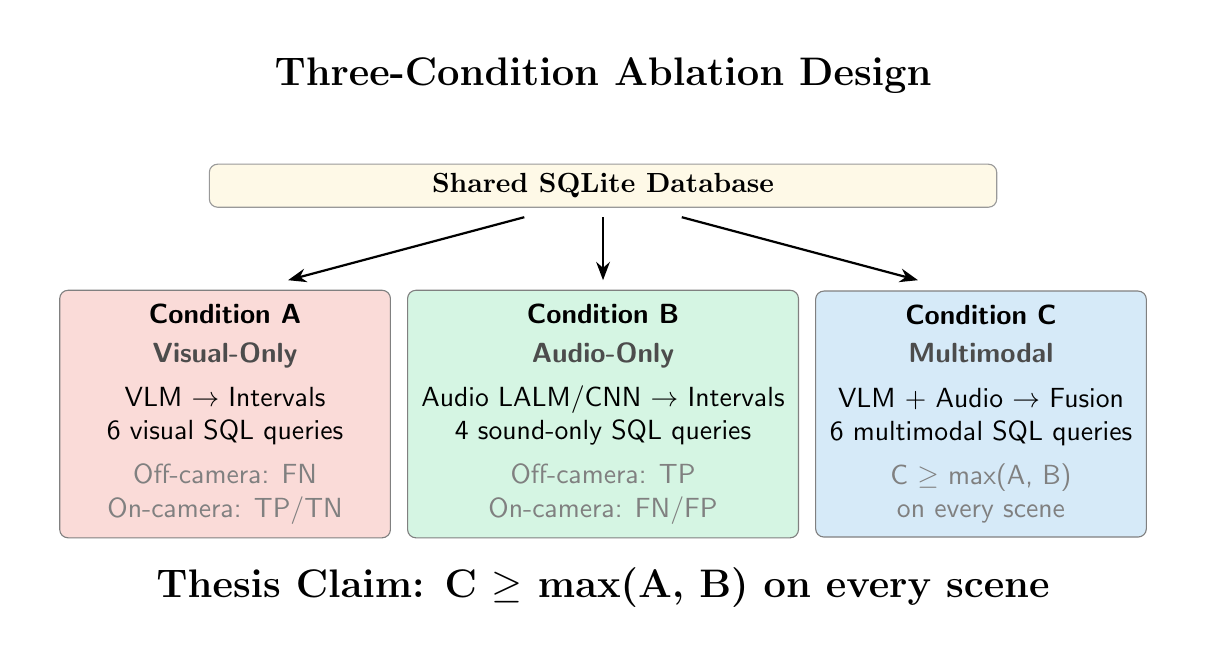
\begin{tikzpicture}[
  every node/.style={font=\sffamily},
  box/.style={draw=black!50, rounded corners=3pt, align=center, inner sep=5pt, minimum width=4.2cm},
  arrow/.style={-Stealth, thick},
]

\draw[white] (-0.3,-0.3) rectangle (14.3,7.5);
\node[font=\Large\bfseries] at (7,6.9) {Three-Condition Ablation Design};

\node[draw=black!40, fill=cYellow, rounded corners=3pt, font=\bfseries, minimum width=10cm, align=center] (db) at (7,5.5) {Shared SQLite Database};

\node[box,fill=cRed] (A) at (2.2,2.6) {
    \textbf{Condition A}\\[2pt]
    \textbf{\textcolor{black!70}{Visual-Only}}\\[4pt]
    VLM $\rightarrow$ Intervals\\6 visual SQL queries\\[4pt]
    \textcolor{black!50}{Off-camera: FN}\\\textcolor{black!50}{On-camera: TP/TN}
};
\node[box,fill=cGreen] (B) at (7.0,2.6) {
    \textbf{Condition B}\\[2pt]
    \textbf{\textcolor{black!70}{Audio-Only}}\\[4pt]
    Audio LALM/CNN $\rightarrow$ Intervals\\4 sound-only SQL queries\\[4pt]
    \textcolor{black!50}{Off-camera: TP}\\\textcolor{black!50}{On-camera: FN/FP}
};
\node[box,fill=cBlue] (C) at (11.8,2.6) {
    \textbf{Condition C}\\[2pt]
    \textbf{\textcolor{black!70}{Multimodal}}\\[4pt]
    VLM + Audio $\rightarrow$ Fusion\\6 multimodal SQL queries\\[4pt]
    \textcolor{black!50}{C $\ge$ max(A, B)}\\\textcolor{black!50}{on every scene}
};

\draw[arrow] (6.0,5.1) -- (3.0,4.3);
\draw[arrow] (7.0,5.1) -- (7.0,4.3);
\draw[arrow] (8.0,5.1) -- (11.0,4.3);

\node[font=\Large\bfseries] at (7,0.4) {Thesis Claim: C $\ge$ max(A, B) on every scene};

\end{tikzpicture}
\end{document}
